\documentclass{beamer}
\setbeamertemplate{caption}[numbered]
\usepackage{phdstyle}

%% image directories
\newcommand{\home}{\string~}
\newcommand{\Artem}{\home/REPOS/COSYINF/img/Artem}
\newcommand{\multisext}{\Artem/multisext_test}
\newcommand{\compare}{\Artem/spin_vs_polarization_fit_comp}
\newcommand{\decoh}{\Artem/decoherence_frequency_dependence}

\title{Spin decoherence in a Frozen Spin lattice, its suppression and effect on the Frequency Domain EDM statistic}
\author{Alexander Aksentev}
\date{\today}

\begin{document}
\begin{frame}
  \titlepage
\end{frame}

\begin{frame}\frametitle{Spin precession essentials}
  \begin{itemize}
  \item T-BMT equation
  \item spin tune and precession axis
  \end{itemize}
\end{frame}

\begin{frame}\frametitle{Spin tune decoherence}
  \begin{itemize}
  \item spin tune expression $\nu_s = \gamma G$
  \item Phase stability principle
  \item orbit lengthening
  \item equilibrium-level momentum shift
  \item effective gamma $\gamma_{eff}$
  \end{itemize}
\end{frame}

\begin{frame}\frametitle{Sextupole decoherence suppression theory}
  \begin{itemize}
  \item orbit length effect
  \item compaction factor effect
  \end{itemize}
\end{frame}

\begin{frame}\frametitle{Simulation setup}
  \begin{itemize}
  \item beam
  \item lattice
  \item tracking parameters
  \item written data
  \end{itemize}
\end{frame}

\begin{frame}\frametitle{Spin precession axis effect}
  \begin{figure}[H]
    \centering
    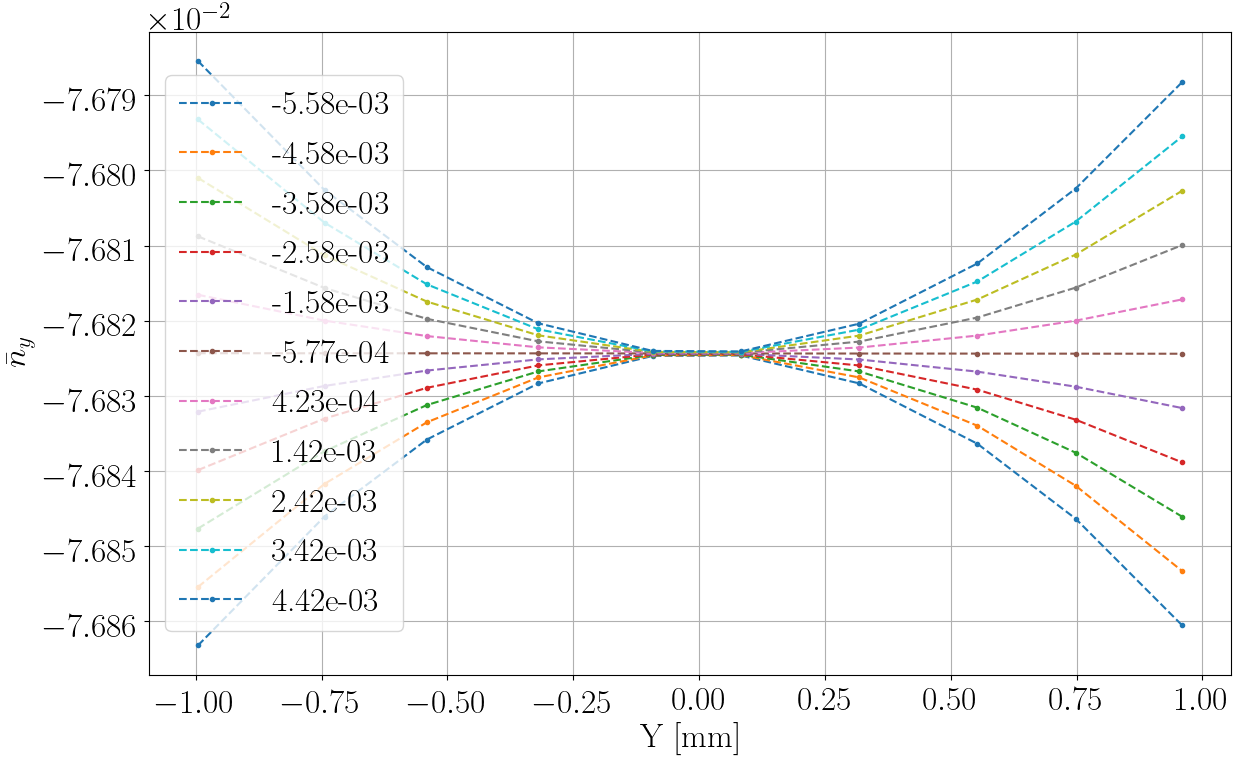
\includegraphics[width=\linewidth]{\multisext/ny_vs_offset}
    \caption{SPA component $\bar n_y$ as a function of the vertical beam offset, sextupole gradient value.\label{fig:DECOH_full_ny}}
  \end{figure}
\end{frame}

\begin{frame}\frametitle{SPA: zoom}
  \begin{figure}[H]
    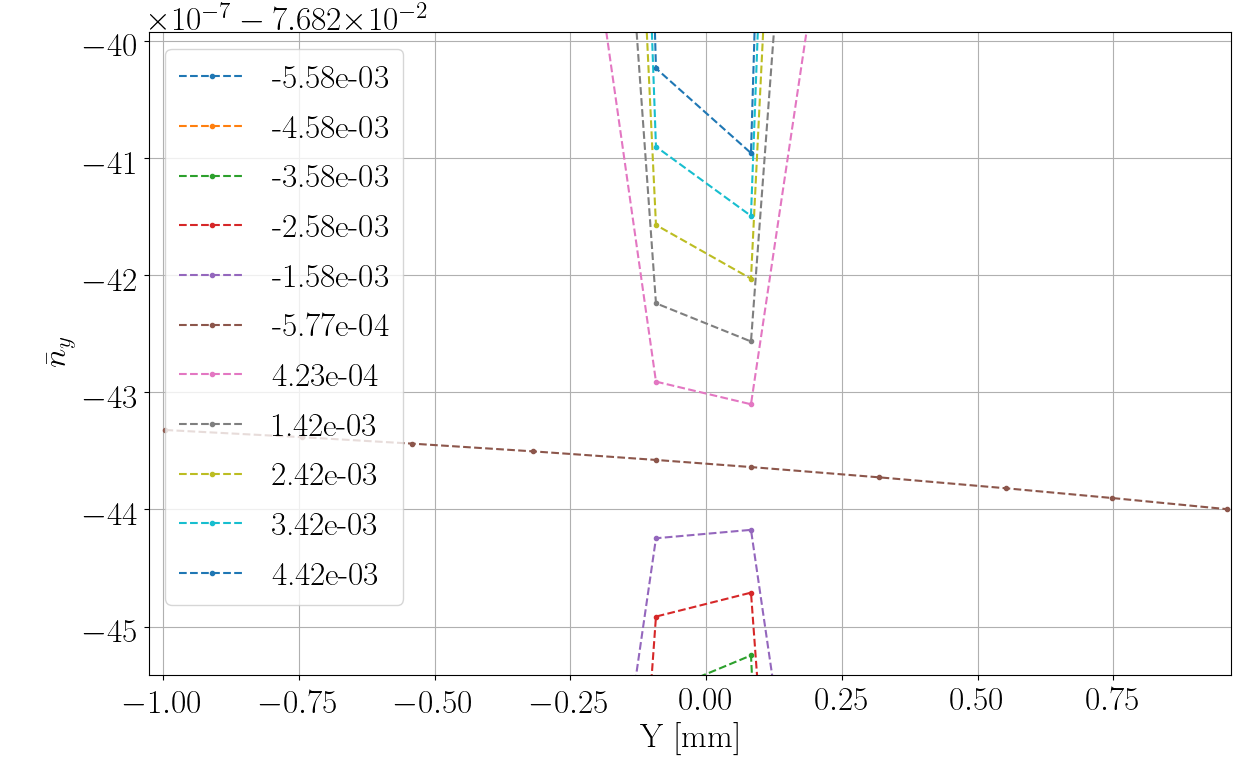
\includegraphics[width=\linewidth]{\multisext/ny_vs_offset_zoom}
    \caption{Zoom of Figure~\ref{fig:DECOH_full_ny}. SPA component $\bar
      n_y$ (as well as $\bar n_x$) is a parabola in the neighborhood of the reference orbit at
      the optimal GSY value, unlike $nu_s$, which is \textbf{linear}.}
  \end{figure}
\end{frame}

\begin{frame}\frametitle{Spin tune effect}
  \begin{figure}[H]
    \centering
    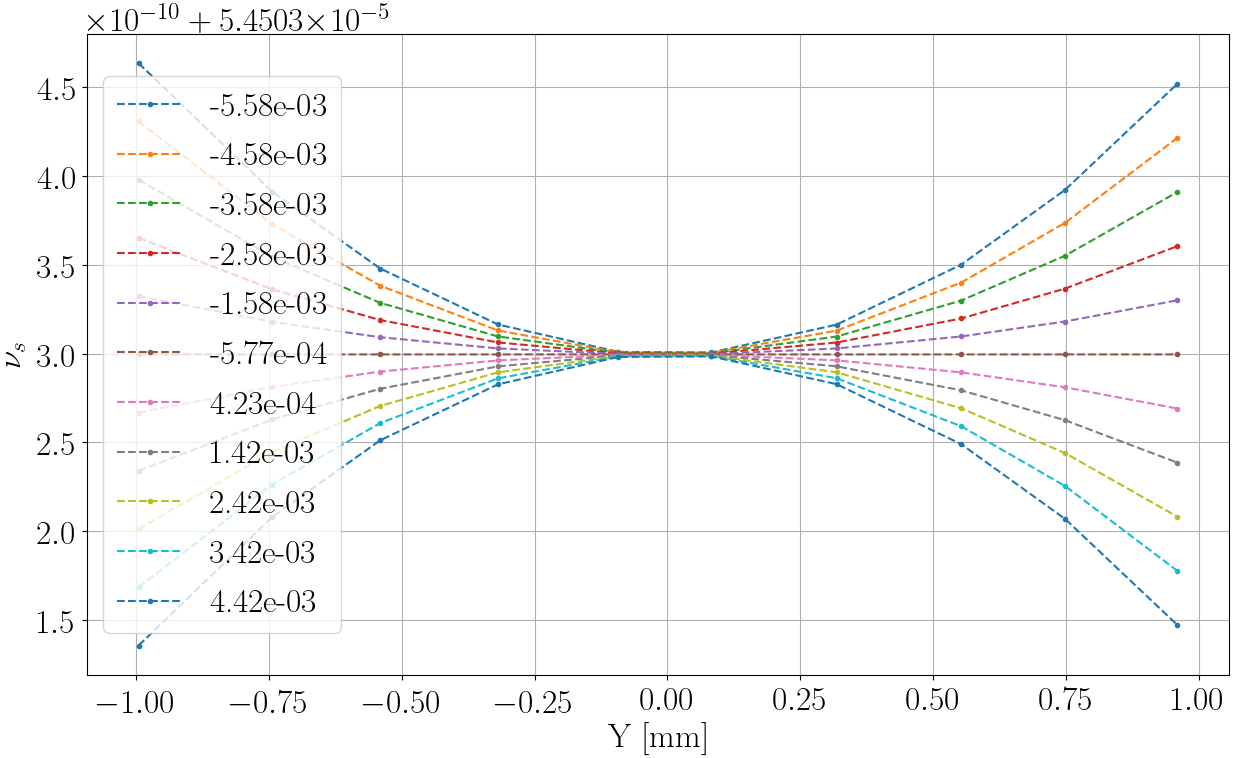
\includegraphics[width=\linewidth]{\multisext/spin_tune_vs_offset}
    \caption{Spin tune $\nu_s$.\label{fig:SpinTune_vs_Y0_GSY}}
  \end{figure}
\end{frame}
\begin{frame}\frametitle{Frequency estimate effect}
  \begin{figure}[H]
    \centering
    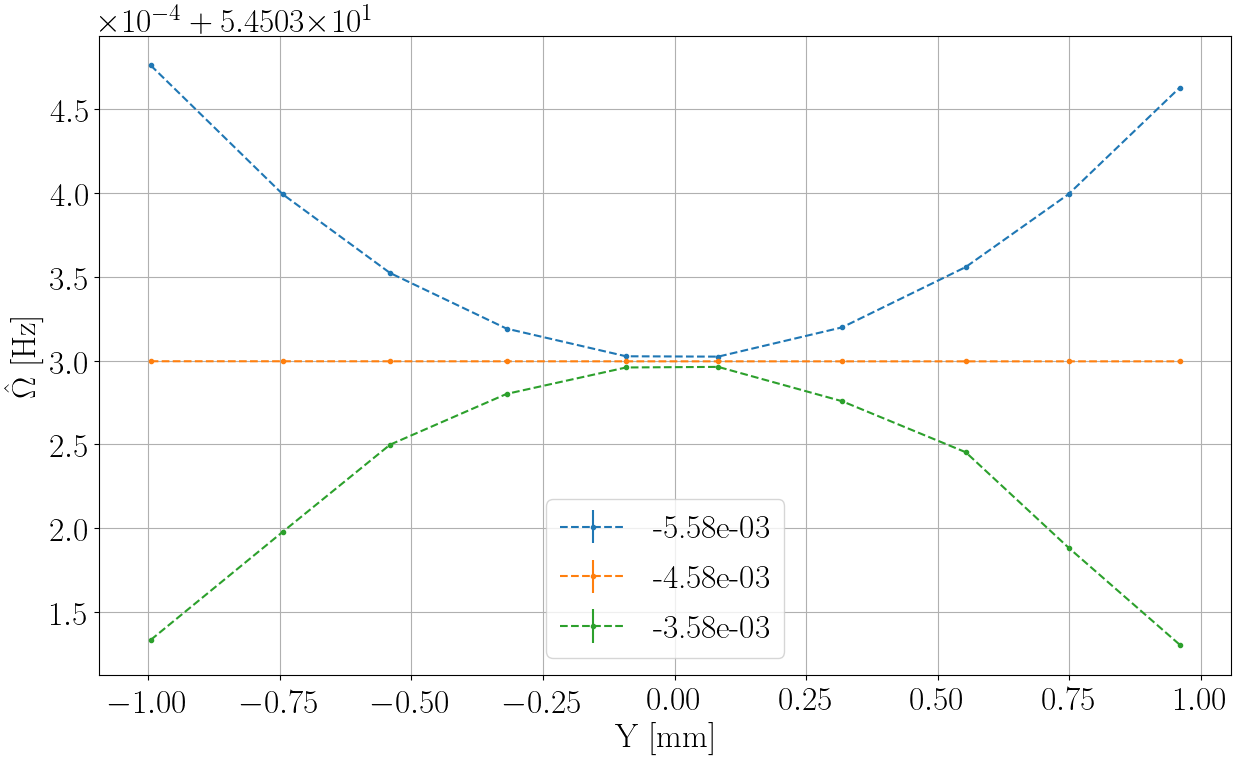
\includegraphics[width=\linewidth]{\multisext/FreqY_vs_offset}
    \caption{Frequency estimate for the optimal sextupole gradient (orange) and the values at the ends of the searched range.\label{fig:FreqY_vs_offset}}
  \end{figure}
\end{frame}
\begin{frame}\frametitle{Frequency estimate: zoom}
  \begin{figure}[H]
    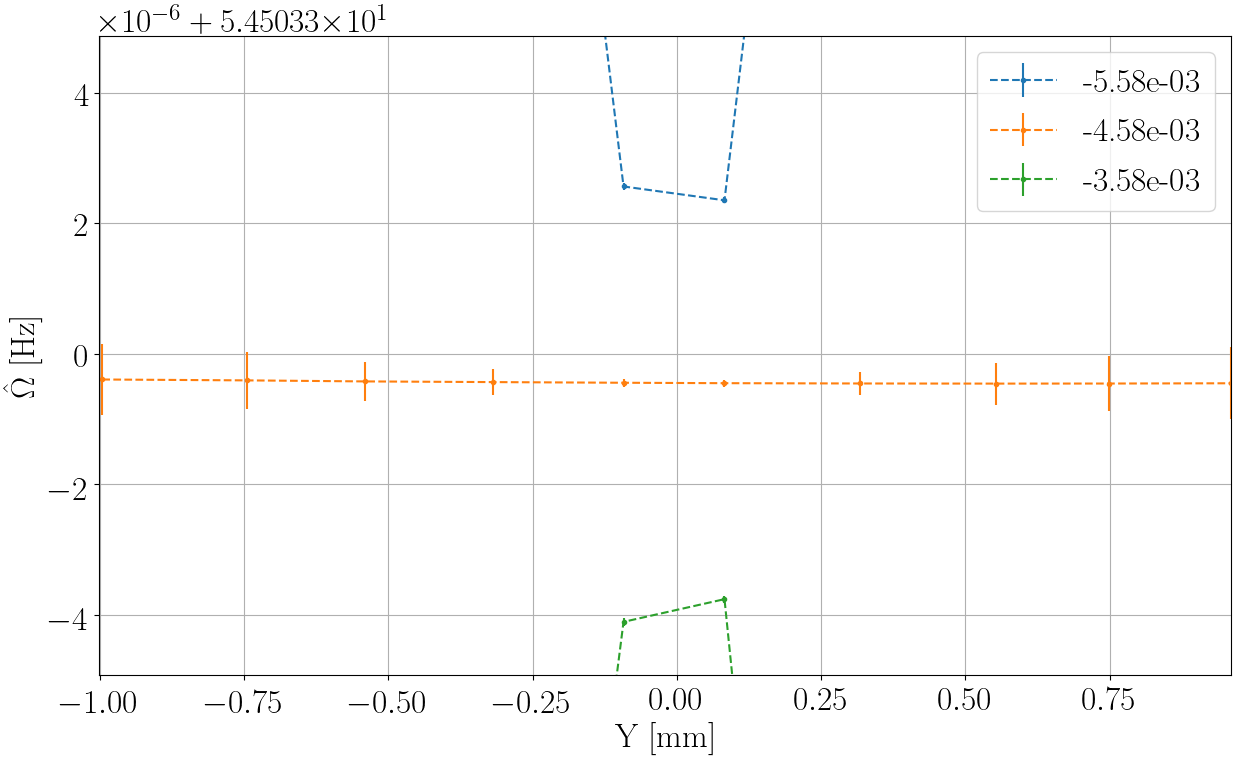
\includegraphics[width=\linewidth]{\multisext/FreqY_vs_offset_zoom}
    \caption{Zoom of Figure~\ref{fig:FreqY_vs_offset}. Frequency estimate depends on the offset value linearly,
      like  $\nu_s$, and unlike $\bar n_y$.}
  \end{figure}
\end{frame}

\begin{frame}\frametitle{ST+SPA structure}
  \begin{figure}[H]
  \centering
  \includegraphics[width=\linewidth]{\decoh/ny_vs_turn}
  \caption{SPA component $\bar n_y$ for \textbf{particles} with offsets:
    [1.02749, 1.02937, 1.02840] mm. We observe small rapid oscillations about
    an average level. This average level changes parabolically with the vertical
    offset (Figure~\ref{fig:mean_tune_axis} below). The rapid oscillations are
    due to betatron motion (Figures~\ref{fig:tune_axis_position_y},
    and~\ref{fig:tune_axis_position_x}).\label{fig:ny_vs_turn}}
\end{figure}
\end{frame}

\begin{frame}
  \begin{figure}[H]
    \centering
    \includegraphics[width=\linewidth]{\decoh/mean_spin_tune_vs_offset}
    \caption{Mean level of spin tune as a function of beam offset}
  \end{figure}
\end{frame}

\begin{frame}
  \begin{figure}[H]
    \includegraphics[width=\linewidth]{\decoh/mean_nbar_vs_mean_spin_tune}
    \caption{Mean SPA and ST levels versus each other. Observe strong correlation.\label{fig:mean_tune_axis}}
  \end{figure}
\end{frame}

\begin{frame}\frametitle{Vertical betatron motion dependence}
  \begin{figure}[H]
    \centering
    \begin{subfigure}[t]{.5\textwidth}
      \includegraphics[width=\linewidth]{\decoh/ny_vs_y}
      \caption{SPA component $\bar n_y$ as a function of the vertical particle position.}
    \end{subfigure}~
    \begin{subfigure}[t]{.5\textwidth}
      \includegraphics[width=\linewidth]{\decoh/spin_tune_vs_y}
      \caption{Spin tune $\nu_s$ as a function of the vertical particle position.}
    \end{subfigure}
    \caption{Particle spin precession frequency depending on its vertical position.
      The observed non-functionality of the parameters on the $y$-position os due to the dependence on the $x$-position as well, which also oscillates at a small amplitude (Figure~\ref{fig:tune_axis_position_x}). \label{fig:tune_axis_position_y}}
  \end{figure}
\end{frame}

\begin{frame}\frametitle{Horizontal betatron motion dependence}
  \begin{figure}[H]
    \centering
    \begin{subfigure}[t]{.5\textwidth}
      \includegraphics[width=\linewidth]{\decoh/ny_vs_x}
      \caption{SPA component $\bar n_y$ as a function of the horizontal particle position.}
    \end{subfigure}~
    \begin{subfigure}[t]{.5\textwidth}
      \includegraphics[width=\linewidth]{\decoh/spin_tune_vs_x}
      \caption{Spin tune $\nu_s$ as a function of the horizontal particle position.}
    \end{subfigure}
    \caption{Particle spin precession frequency as a function of itsd radial position.\label{fig:tune_axis_position_x}}
  \end{figure}
\end{frame}
\end{document}
